\documentclass{standalone}
\usepackage{pgfplots}
\pgfplotsset{compat=newest}

\begin{document}
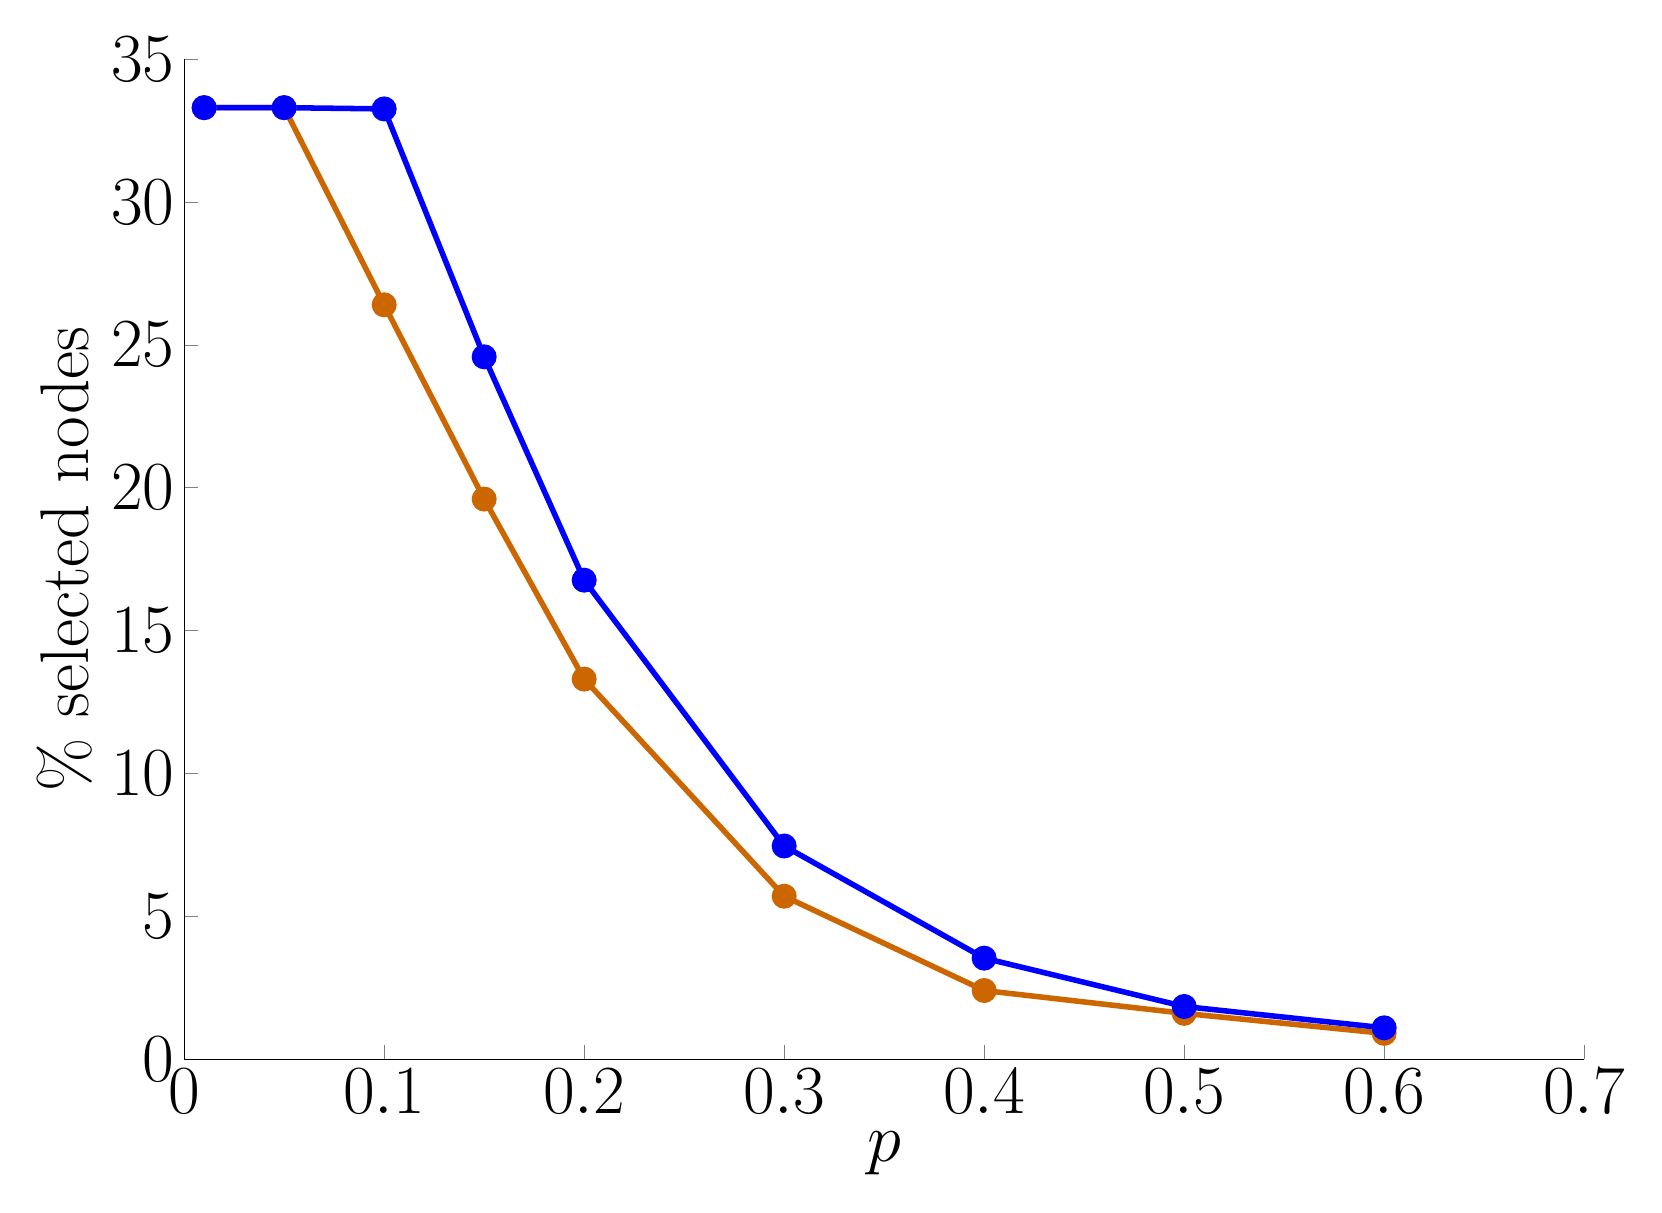
\begin{tikzpicture}

\begin{axis}[%
tick label style={font=\Huge},
label style={font=\Huge},
legend style={font=\Huge},
view={0}{90},
width=7in,
height=5in,
scale only axis,
xmin=0, xmax=0.7,
xtick={0, 0.1, 0.2, 0.3, 0.4, 0.5, 0.6, 0.7},
xlabel={$p$},
ymin=0, ymax=35,
ytick={0, 5, 10, 15, 20, 25, 30, 35},
ylabel={$\%$ selected nodes},
major tick length=5pt,
axis lines*=left,
legend cell align=left,
clip=false]

\addplot [
mark=*,
mark size=3.5pt,
color=orange!80!black,
solid,
line width=2pt,
]
coordinates{
(0.01,33.3)(0.05,33.3)(0.1,26.4)(0.15,19.6)(0.2,13.3)(0.3,5.7)(0.4,2.4)(0.5,1.6)(0.6,0.9)
};

\addplot [
mark=*,
mark size=3.5pt,
color=blue,
solid,
line width=2pt,
]
coordinates{
(0.01,33.3)(0.05,33.3)(0.1,33.256)(0.15,24.579)(0.2,16.762)(0.3,7.458)(0.4,3.533)(0.5,1.841)(0.6,1.094)
};

\end{axis}
\end{tikzpicture}
\end{document}
